\chapter{Critical Path and Delay Analysis in Construction Projects}
\section{Kroll Expert Services}
With experience spanning global industries across the world's continents, we are a market leader for expert witnesses, dispute resolution, advisory and investigative services. Our clients include international contractor, government agencies, blue chip multinationals, investors, developers, banks and insurers.
\begin{itemize}
    \item Delay analysis
          \begin{itemize}
              \item The assessment of the incidence, extent and causes of delay to the progress and completion of capital investment projects
          \end{itemize}
    \item Quantum analysis
          \begin{itemize}
              \item Construction quantum is the assessment of financial entitlement of the parties arising from claims under or out of a construction contract
          \end{itemize}
    \item Project advisory
          \begin{itemize}
              \item Our advisory practice draws on our in-depth project delivery, management and industry expert insight to provide pre-dispute advisory services to capital projects, infrastructure programmes and real assets organisations across their delivery lifecycle
          \end{itemize}
\end{itemize}
\section{Dispute in construction and the role of experts}
\subsection{What is a dispute?}
\begin{figure}[H]
    \centering
    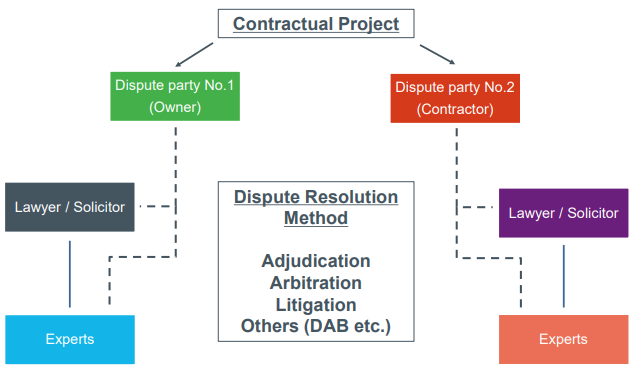
\includegraphics[width = 0.8\textwidth]{img/figure27.png}
    \caption{Dispute pathway.}
\end{figure}
\subsection{Typical sequence to a trial}
\begin{enumerate}
    \item Dispute arises between two parties
    \item Dispute party hires a lawyer
    \item Lawyer engages with an independent expert
    \item Dispute party provides the expert with evidence
          \begin{itemize}
              \item Identify issues
              \item Analyse data
              \item Prioritise key areas
          \end{itemize}
    \item The expert provides independent expert report
          \begin{itemize}
              \item Report could be used:
              \item in dispute resolution
              \item for consulting purposes
              \item for negotiation purposes
          \end{itemize}
    \item Engage with opposing expert
    \item Go to trial
          \begin{itemize}
              \item Oral evidence / cross examination
          \end{itemize}
\end{enumerate}
\subsection{Independent expert}
\begin{itemize}
    \item Independent
          \begin{itemize}
              \item An expert witness is to provide \textbf{independent}, impartial and unbiased evidence to the court or tribunal
          \end{itemize}
    \item Expert
          \begin{itemize}
              \item An \textbf{expert} is a person engages to give an opinion based on experience, knowledge and expertise
          \end{itemize}
    \item Assist
          \begin{itemize}
              \item The primary duty of an expert witness is to \textbf{assist} the court
          \end{itemize}
\end{itemize}
\section{Critical path and delay analysis}
\subsection{What is delay analysis?}
Definition:
\begin{quoting}
    Delay analysis is the assessment of impact, \textbf{causes} and \textbf{effects} of a construction or engineering project not meeting its original forecast completion date.
\end{quoting}
Delay analysis includes:
\begin{itemize}
    \item Determination of critical path of the project (EFFECT)
    \item Assessment of extent of delays (quantification of EFFECT)
    \item Assessment of causes of delays (CAUSE)
\end{itemize}
\subsection{What is the critical path?}
\begin{quoting}
    The longest sequence of activities through a project network from start to finish, the sum of whose durations determines the overall project duration.
\end{quoting}
\subsection{Basics of delay}
\begin{figure}[H]
    \centering
    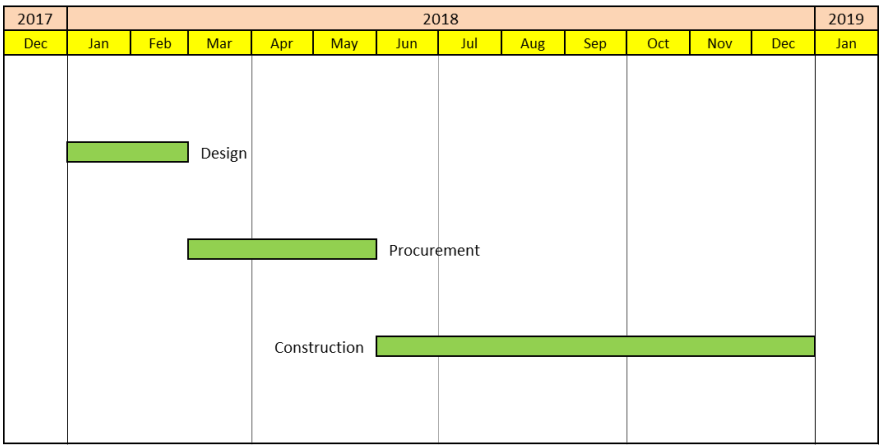
\includegraphics[width = 0.8\textwidth]{img/figure28.png}
    \caption{Work programmes can be as simple as a few bar charts.}
\end{figure}
\begin{figure}[H]
    \centering
    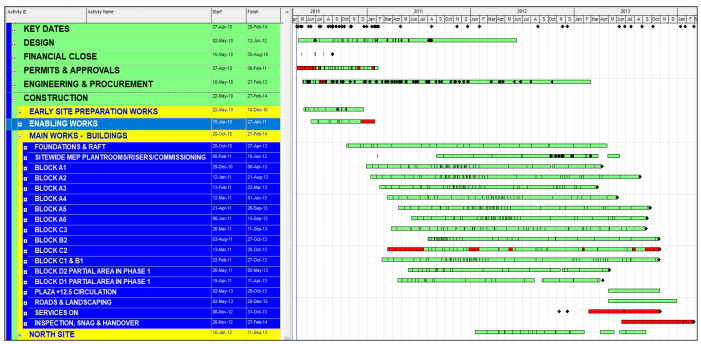
\includegraphics[width = 0.8\textwidth]{img/figure29.png}
    \caption{Or a complex schedule prepared in a specialist software.}
\end{figure}
\subsection{Information sources}
Experts do not just rely on the programme. The best intelligently utilise other as-built evidence. A key rule:
\begin{quoting}
    Never rely on assumptions when you know the facts.
\end{quoting}
\begin{itemize}
    \item Primary
          \begin{itemize}
              \item Photographs
              \item Videos
              \item Site diaries / daily reports
              \item Pour / installation records
              \item Inspection sheets
              \item Daily allocation sheets L/P/M
              \item Detailed timesheets / labour resources timesheets
              \item Detailed sign-off sheets
              \item Detailed quality records
              \item Contemporaneously marked-up progress drawings
              \item Quality Assurance documentation
          \end{itemize}
    \item Secondary
          \begin{itemize}
              \item Updated programmes
              \item Look-ahead programmes
              \item Progress reports
              \item Progress meetings' minutes
              \item Data spreadsheets
              \item Valuations / earned value analysis
              \item As-built drawings / records
              \item Claims
          \end{itemize}
    \item Tertiary
          \begin{itemize}
              \item Correspondence
              \item General meeting minutes
              \item RFIs (Request for Inspections)
              \item TQs (Technical Queries)
              \item Variations / Changes of Orders
              \item Instructions
              \item Etcetera
          \end{itemize}
\end{itemize}
\subsection{Methods of delay analysis}
\begin{table}[H]
    \centering
    \begin{tabular}{@{}llll@{}}
        \toprule
        \textbf{Method of analysis}             & \textbf{Analysis type} & \textbf{Critical path determined} & \textbf{Delay impact determined} \\
        \midrule
        Impacted as-planned analysis            & Cause \& Effect        & Prospectively                     & Prospectively                    \\
        Time impact analysis                    & Cause \& Effect        & Contemporaneously                 & Prospectively                    \\
        Time slice windows analysis             & Effect \& Cause        & Contemporaneously                 & Retrospectively                  \\
        As-planned vs as-built windows analysis & Effect \& Cause        & Contemporaneously                 & Retrospectively                  \\
        Longest path analysis                   & Effect \& Cause        & Retrospectively                   & Retrospectively                  \\
        Collapsed as-built analysis             & Cause \& Effect        & Retrospectively                   & Retrospectively                  \\
        \bottomrule
    \end{tabular}
    \caption{Methods of delay analysis.}
\end{table}
\subsection{Example 1}
Consider two buildings:
\begin{figure}[H]
    \centering
    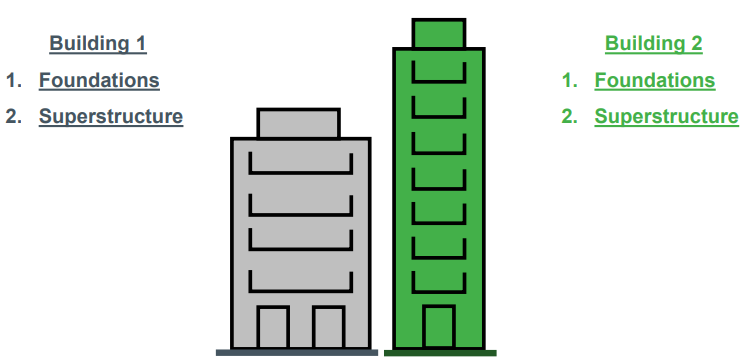
\includegraphics[width = 0.8\textwidth]{img/figure30.png}
    \caption{Example project with two buildings.}
\end{figure}
\subsubsection{Impact as-planned analysis}
Potential issue with the result we get as it is all perspective. None of the sequence happened as it should have. Everything in green is a projection i.e. what should have happened. Impacting what should happen is not consistent with the real world events. For example, in this example, we could add mitigation to the superstructure of B2, moving the project completion to the left (shortening it).

Another issue is that results are quite biased. Using this method, we tend to maximise the impact of delay, so any introduction of a delay event is likely to cause a delay in the completion date, regardless of whether it is critical or not. We have not found a true critical path to impact the delay onto it.

Another issue is that we are only picking certain delay events and not necessarily taking into account other delay events. In this example, we have only taken a delay event for B2. There could be other things happening in B1 that we are not taking into account. This analysis tends to favour the party selecting the events to be modelled; it could be ignoring delay events that are not favourable to the client or the contractor.
\begin{figure}[H]
    \centering
    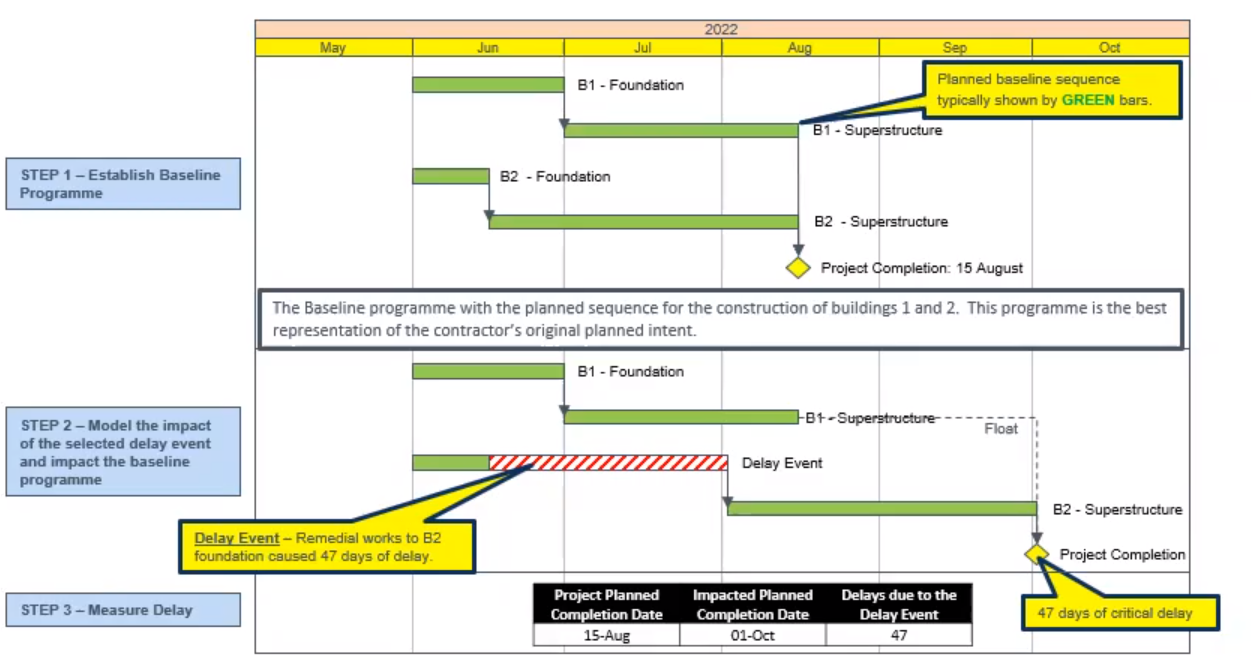
\includegraphics[width = \textwidth]{img/figure31.png}
    \caption{Impact as-planned analysis for example project.}
\end{figure}
\subsubsection{Time impact analysis}
This differs from Impact as-planned analysis, as we take into consideration actual progress on the project, represented by the blue bars. Similarly to the previous analysis method, it is still a matter of perspective. We are still projecting the completion date. Again, we can pick certain delay events that are not necessarily taking into account the full impact of other delay events on the other buildings. However, this analysis method is reliable in anticipating the potential delay of an event. This is a method used on live projects that have not been finished yet to predict delay impact.
\begin{figure}[H]
    \centering
    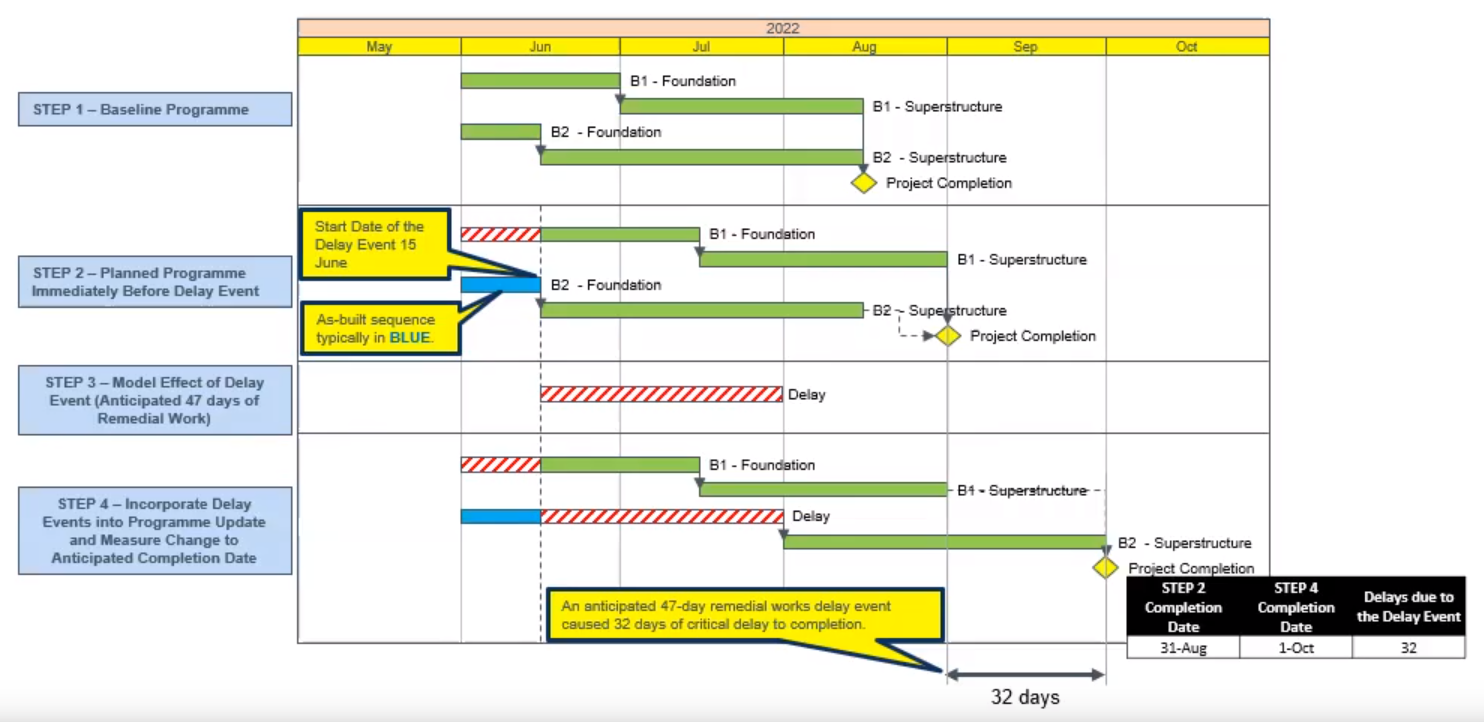
\includegraphics[width = \textwidth]{img/figure32.png}
    \caption{Time impact analysis for example project.}
\end{figure}
\subsubsection{Time slice windows analysis}
This method takes into account all that happened during the project. It takes into account all the ongoing parallel issues and makes an assessment of whether it is critical or not. It is quite an accurate method of delay and is used on projects. An issue is that it relies very heavily on programme updates. This could mean it is heavily biased; in the construction programme the contractor may use it to artificially establish an entitlement for an extension of time. This means that the information provided could be skewed to favour the contractor. In ideal circumstances, when we have an ideal programme and we find it is not biased or it has not been used at all by the contractor, we can use this form of analysis, to analyse delay. However, the case is usually that they are not reliable.
\begin{figure}[H]
    \centering
    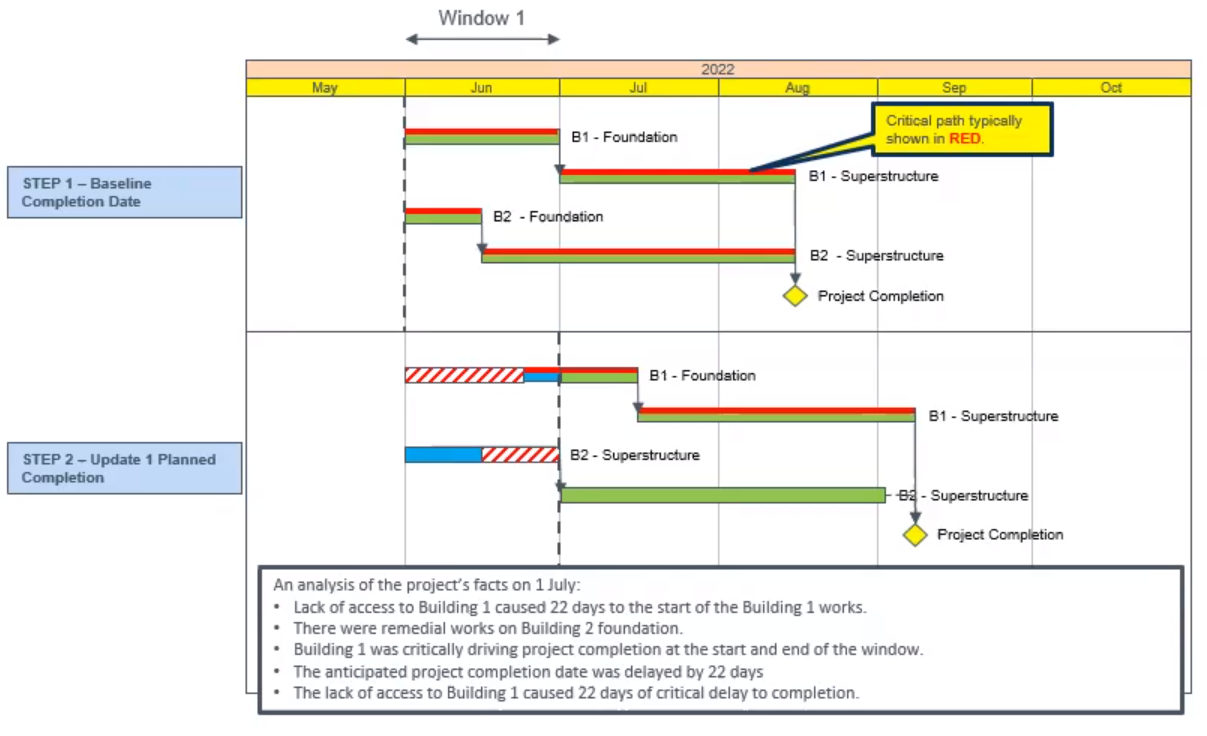
\includegraphics[width = \textwidth]{img/figure33.png}
    \caption{Time slice windows analysis for example project. Window 1}
\end{figure}
\begin{figure}[H]
    \centering
    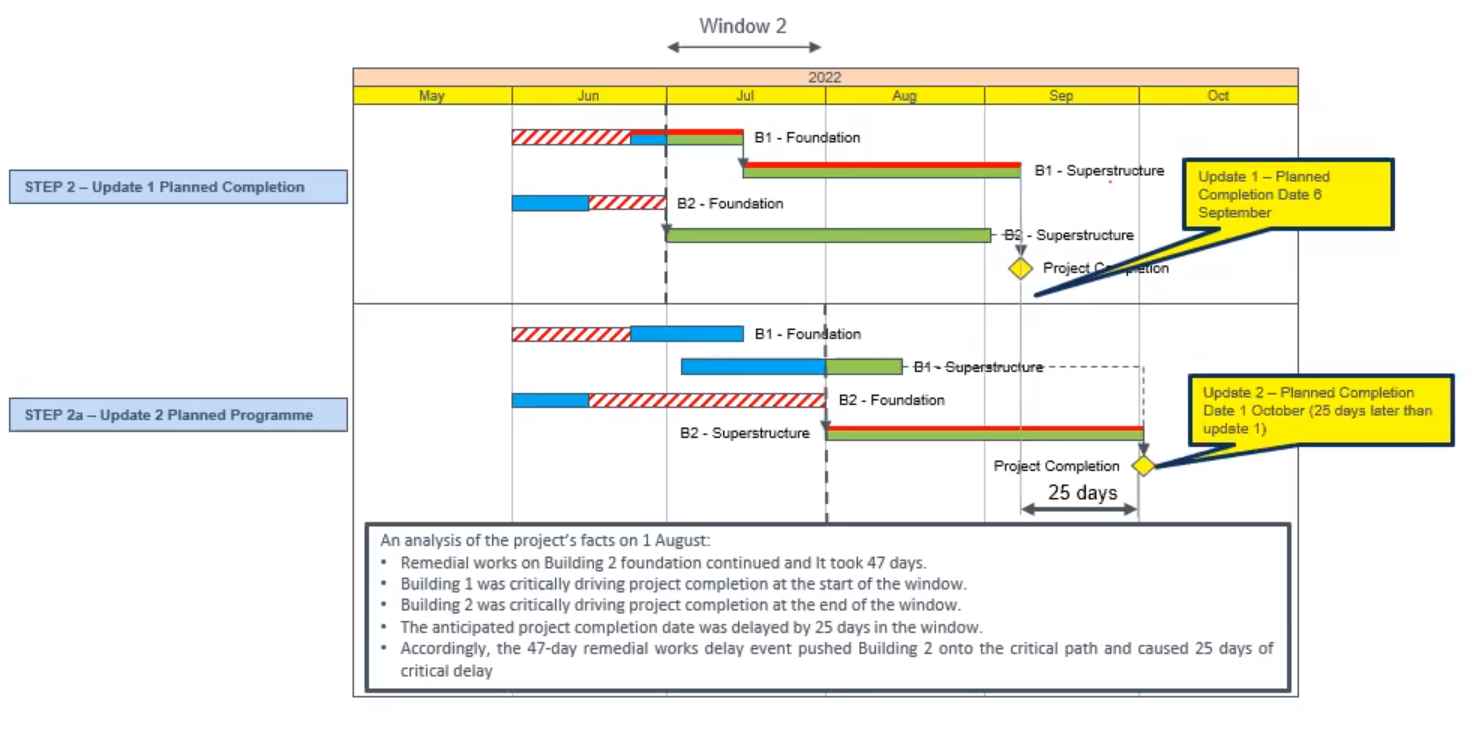
\includegraphics[width = \textwidth]{img/figure34.png}
    \caption{Time slice windows analysis for example project. Window 2.}
\end{figure}
\begin{figure}[H]
    \centering
    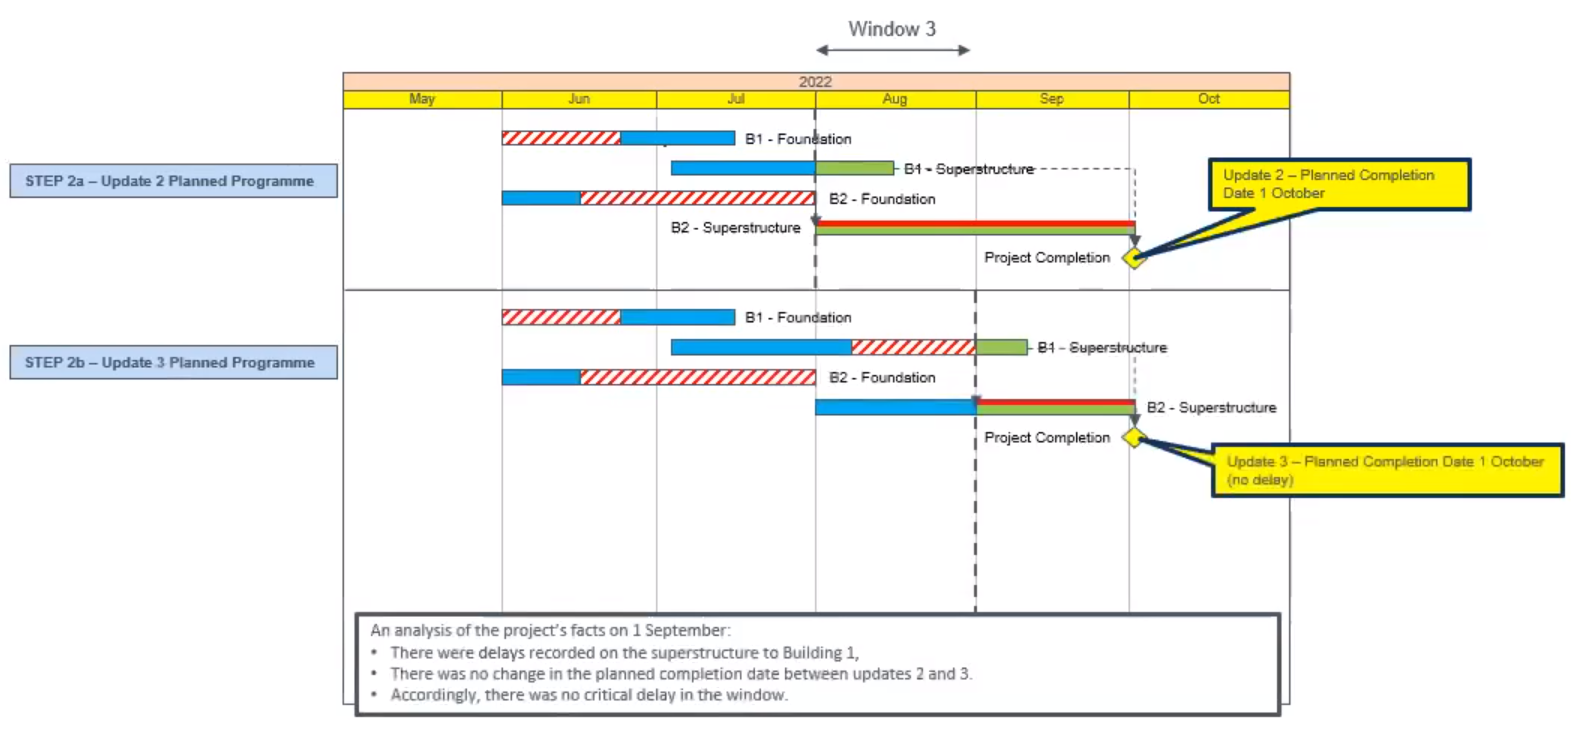
\includegraphics[width = \textwidth]{img/figure35.png}
    \caption{Time slice windows analysis for example project. Window 3.}
\end{figure}
\begin{figure}[H]
    \centering
    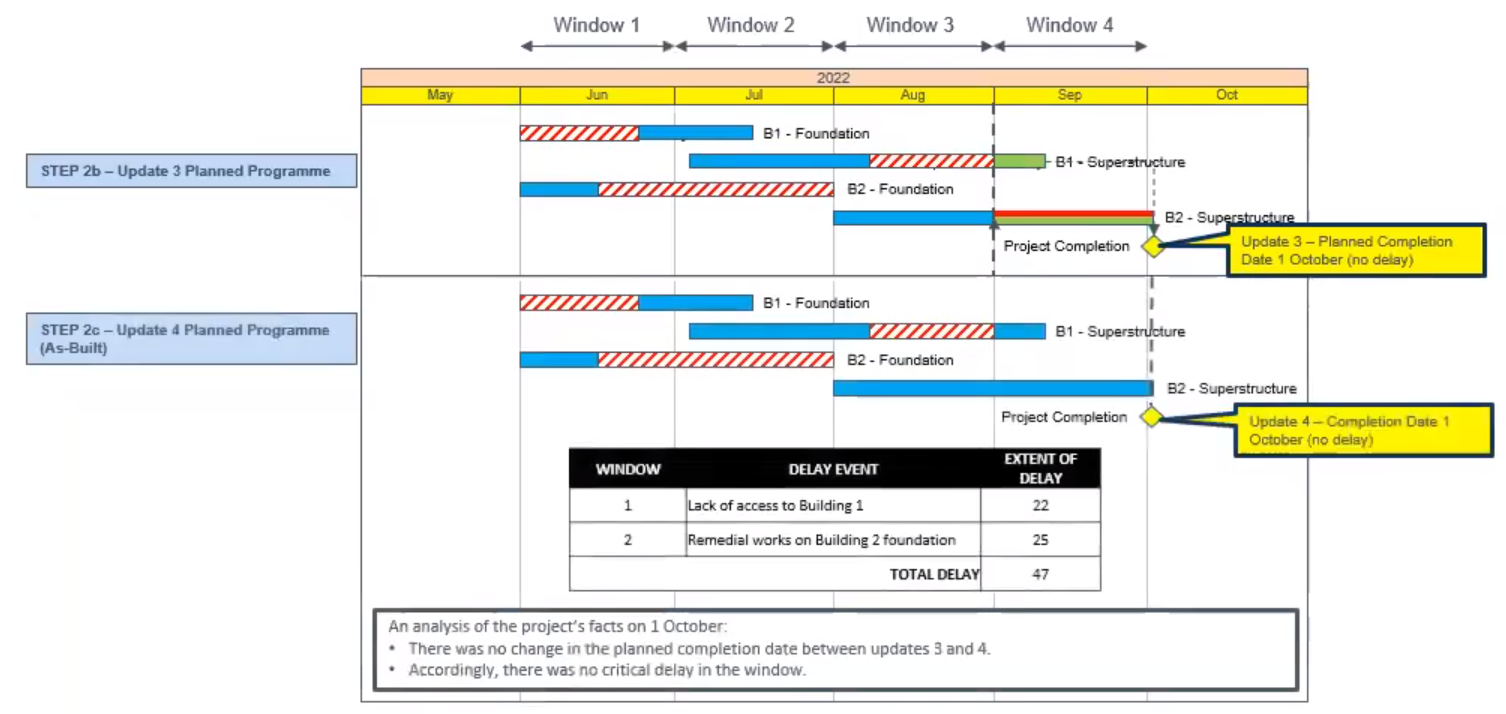
\includegraphics[width = \textwidth]{img/figure36.png}
    \caption{Time slice windows analysis for example project. Window 4.}
\end{figure}
\subsubsection{As-planned vs as-built windows analysis}
More effort is required for this analysis. This is usually the best method to use, however a key issue with this method is that all delays are measured against the baseline programme. This can lead to dispute if the baseline programme is quite wrong and unfeasible. A skewed baseline programme would lead to skewed delay results.

This method of analysis defines the critical path through experience and looking through the data, which is something more difficult to defend, because as an expert, you are relying your own subjective opinion to determine the critical path. Lawyers or disputing parties may argue against this. It also requires the project data to be reliable.
\begin{figure}[H]
    \centering
    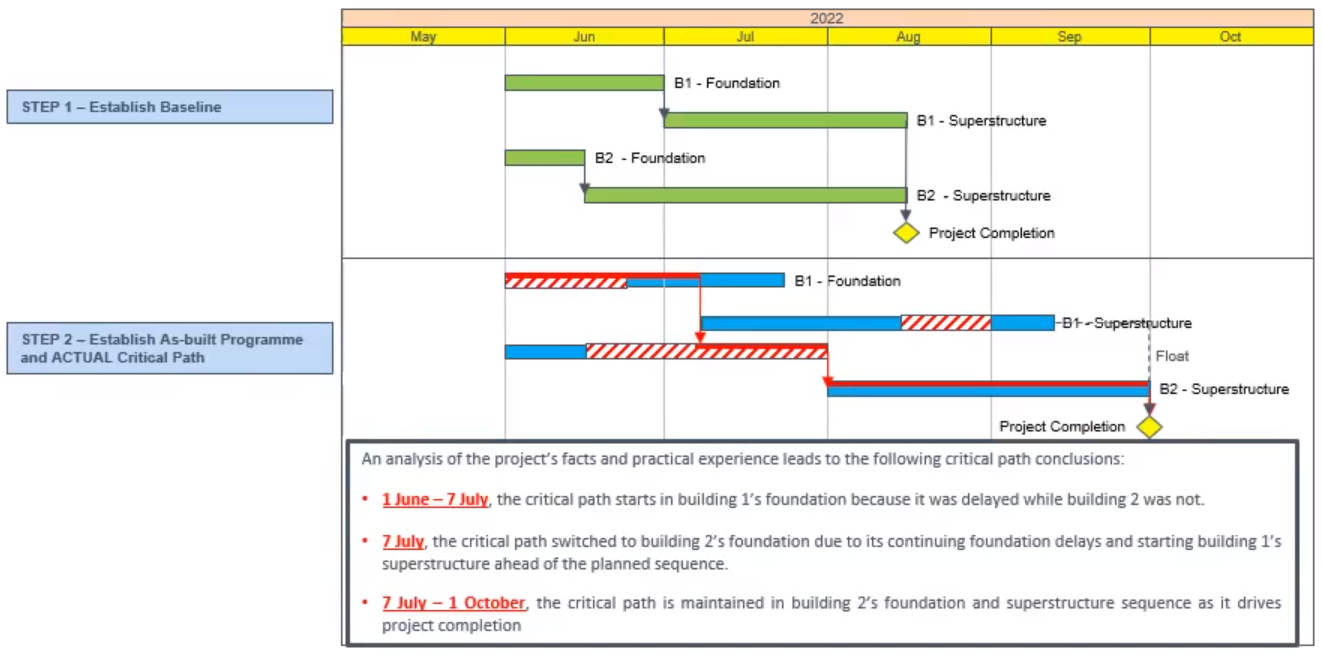
\includegraphics[width = \textwidth]{img/figure37.png}
    \caption{As-planned vs as-built windows analysis for example project. Step 1 \& 2.}
\end{figure}
\begin{figure}[H]
    \centering
    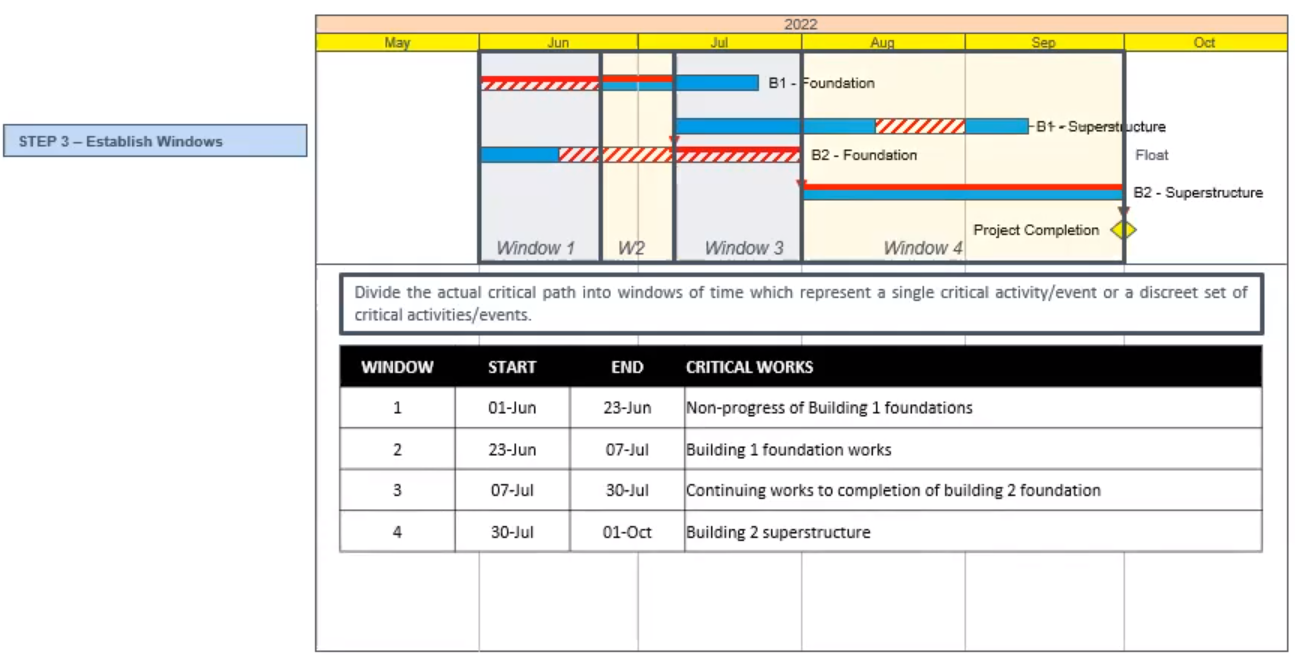
\includegraphics[width = \textwidth]{img/figure38.png}
    \caption{As-planned vs as-built windows analysis for example project. Step 3.}
\end{figure}
\begin{figure}[H]
    \centering
    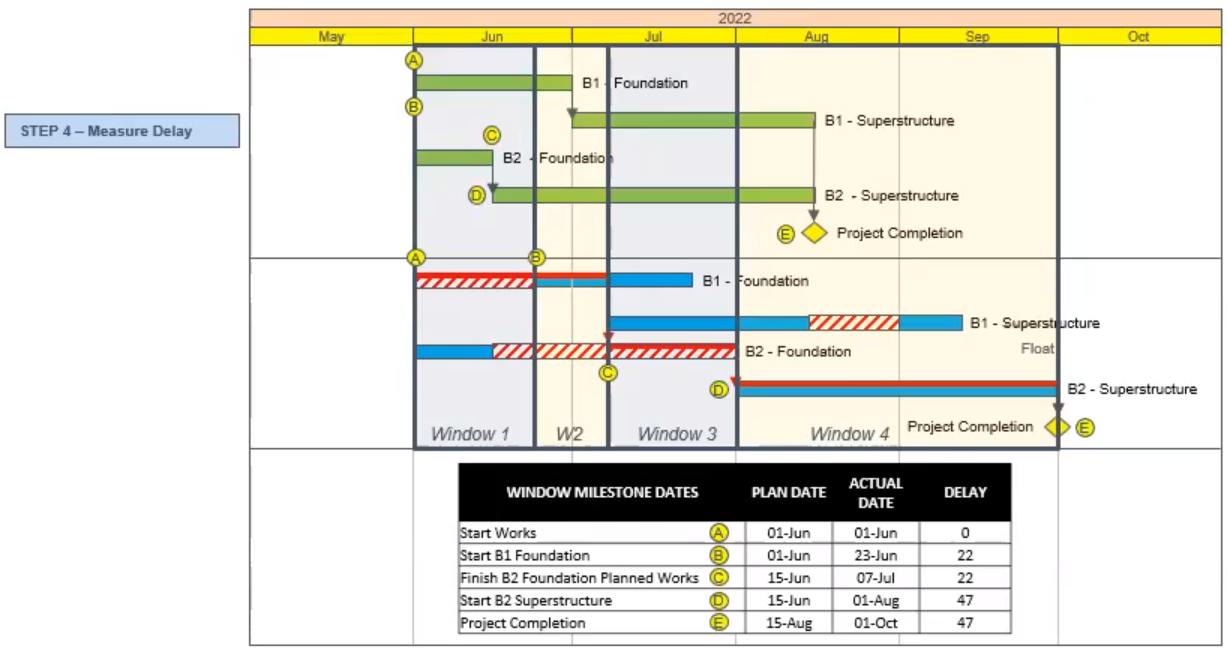
\includegraphics[width = \textwidth]{img/figure39.png}
    \caption{As-planned vs as-built windows analysis for example project. Step 4.}
\end{figure}
\begin{figure}[H]
    \centering
    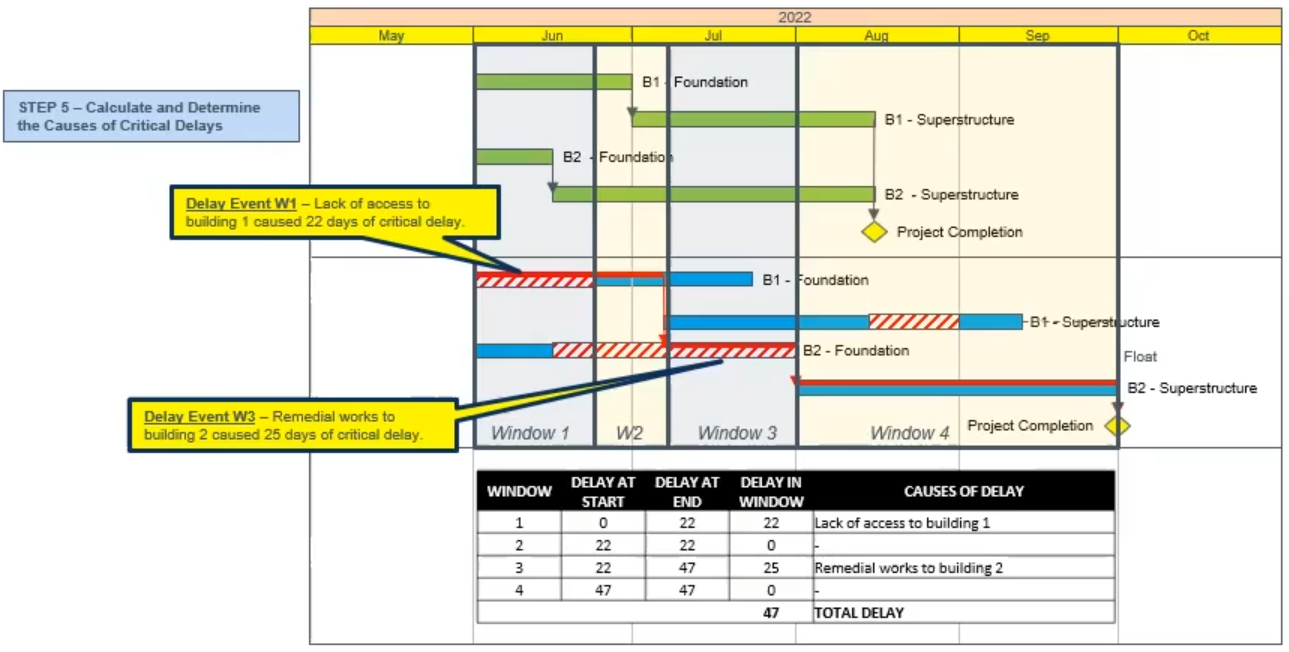
\includegraphics[width = \textwidth]{img/figure40.png}
    \caption{As-planned vs as-built windows analysis for example project. Step 5.}
\end{figure}
\subsubsection{Longest path analysis}
Here, the critical path is found retrospectively, which does not really allow for the switching of the critical path between the two buildings. Usually, in large projects, the critical path switches between many different aspects of the project. In a simple project, this type of analysis might work. For larger projects, we do need to analyse the critical path more contemporaneously. This method of analysis is sometimes used when programme updates are too few or unreasonable, which prevents the use of time slice windows.
\begin{figure}[H]
    \centering
    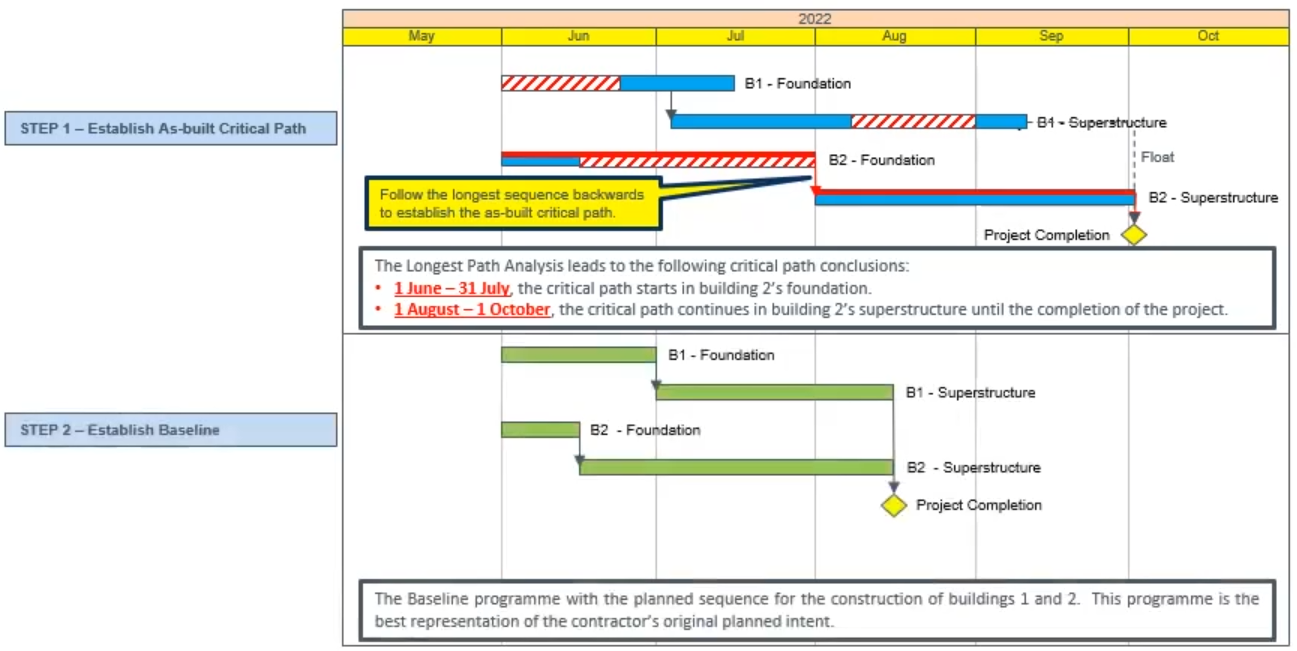
\includegraphics[width = \textwidth]{img/figure41.png}
    \caption{Longest path analysis for example project. Step 1 \& 2.}
\end{figure}
\begin{figure}[H]
    \centering
    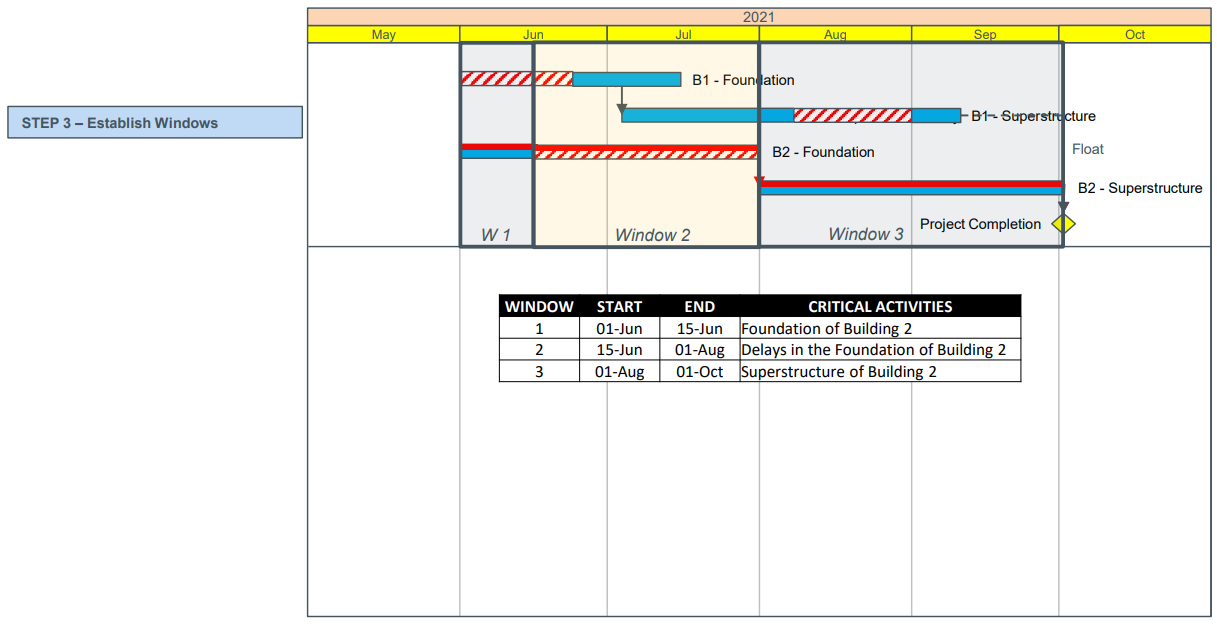
\includegraphics[width = \textwidth]{img/figure42.png}
    \caption{Longest path analysis for example project. Step 3.}
\end{figure}
\begin{figure}[H]
    \centering
    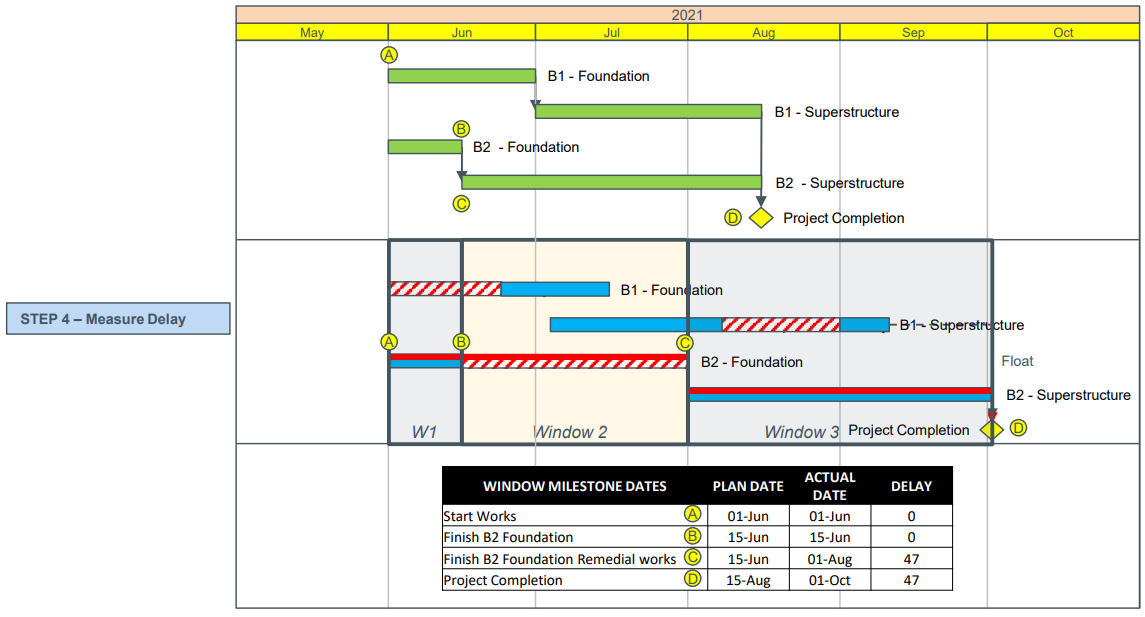
\includegraphics[width = \textwidth]{img/figure43.png}
    \caption{Longest path analysis for example project. Step 4.}
\end{figure}
\begin{figure}[H]
    \centering
    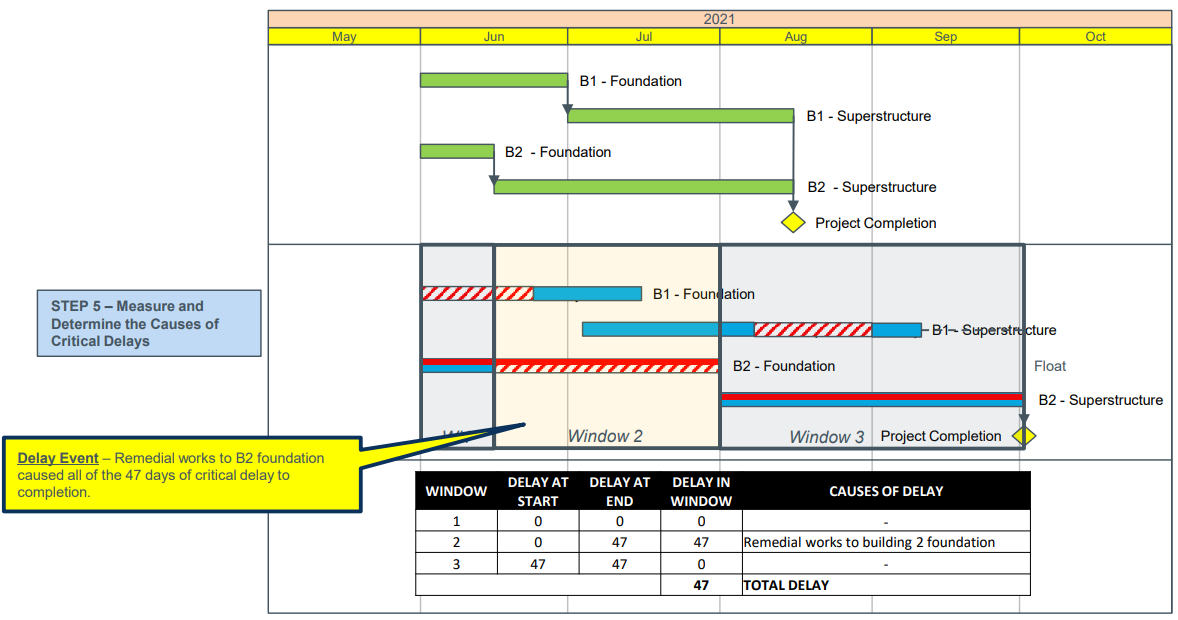
\includegraphics[width = \textwidth]{img/figure44.png}
    \caption{Longest path analysis for example project. Step 5.}
\end{figure}
\subsubsection{Collapsed as-built analysis}
This involves building a programme from scratch using the project records (as-built data) and track what happened in the project. Then we can add in our delay events, and calculate the projected completion date if there was no delay.
\begin{figure}[H]
    \centering
    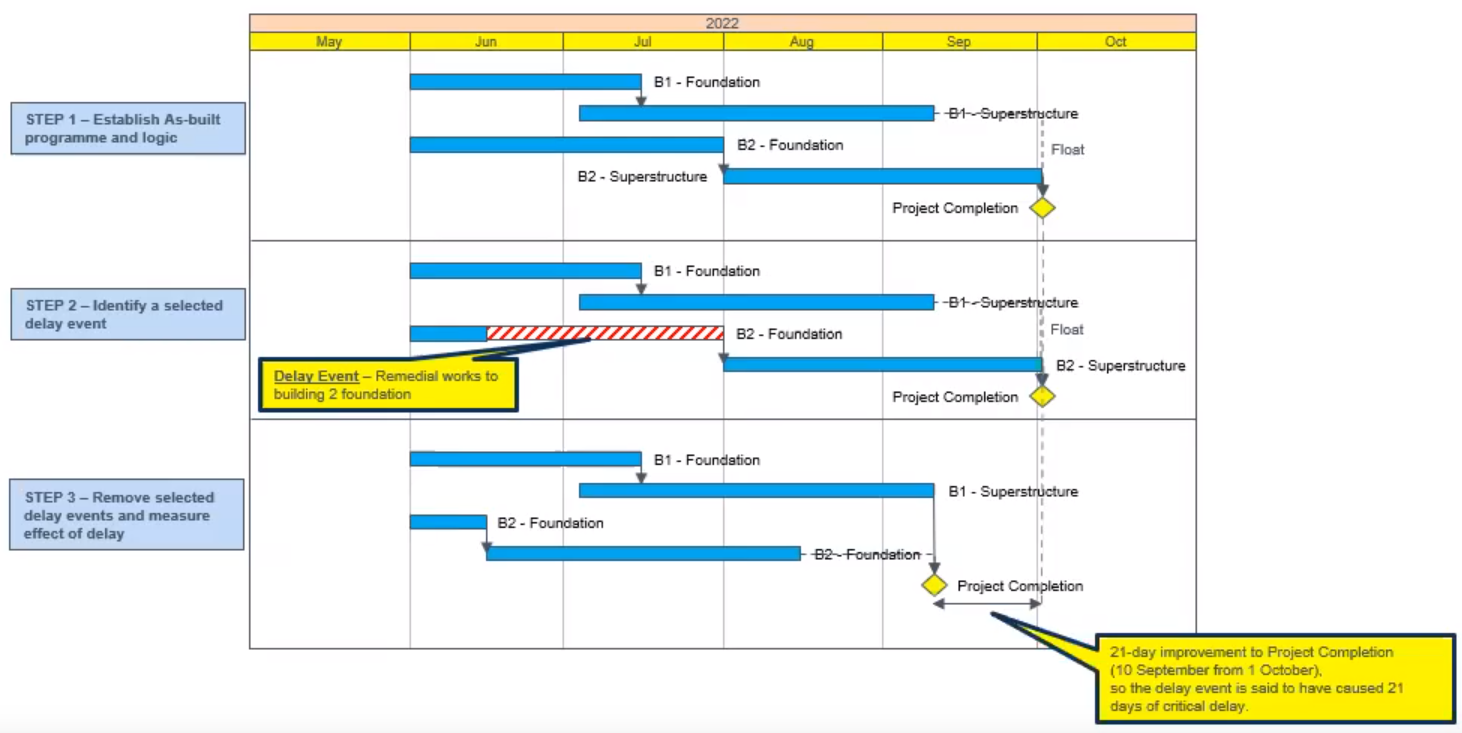
\includegraphics[width = \textwidth]{img/figure45.png}
    \caption{Collapsed as-built analysis for example project.}
\end{figure}
\subsection{Why so many methods?}
Blame lawyers and claims consultants.
\begin{table}[H]
    \centering
    \begin{tabular}{@{}ll@{}}
        \toprule
        \textbf{Method of analysis}             & \textbf{The question it answers}                                           \\
        \midrule
        Impacted as-planned analysis            & What effect would this event(s) have had on the completion date            \\
                                                & assuming everything else went exactly as planned in the programme?         \\
        Time impact analysis                    & What was the likely effect of this event(s) on the completion date         \\
                                                & adjudged from the point in time it was instructed or arose?                \\
        Time slice windows analysis             & What was the contemporaneous or actual critical path to completion         \\
                                                & throughout the works and what were the causes of delay thereto?            \\
        As-planned vs as-built windows analysis & What was the contemporaneous or actual critical path to completion         \\
                                                & throughout the works and what were the causes of delay?                    \\
        Longest path analysis                   & What was the as-built critical path to completion, viewed retrospectively, \\
                                                & and what were the causes of delay thereto?                                 \\
        Collapsed as-built analysis             & But for the event(s) when would the completion date have been achieved?    \\
        \bottomrule
    \end{tabular}
    \caption{Justification for various methods of analysis.}
\end{table}
\subsection{Example 2}
\begin{figure}[H]
    \centering
    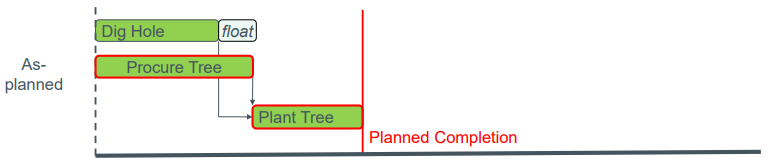
\includegraphics[width = \textwidth]{img/figure46.png}
    \caption{A simple project programme.}
\end{figure}
\begin{figure}[H]
    \centering
    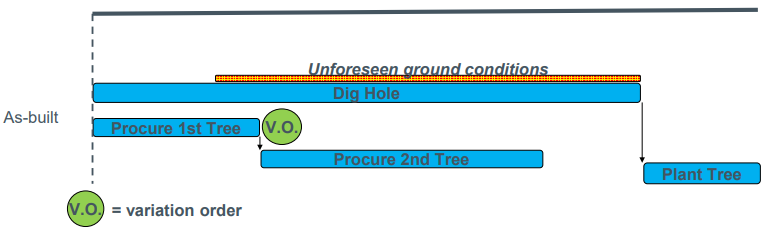
\includegraphics[width = \textwidth]{img/figure47.png}
    \caption{Actual programme.}
\end{figure}
\begin{figure}[H]
    \centering
    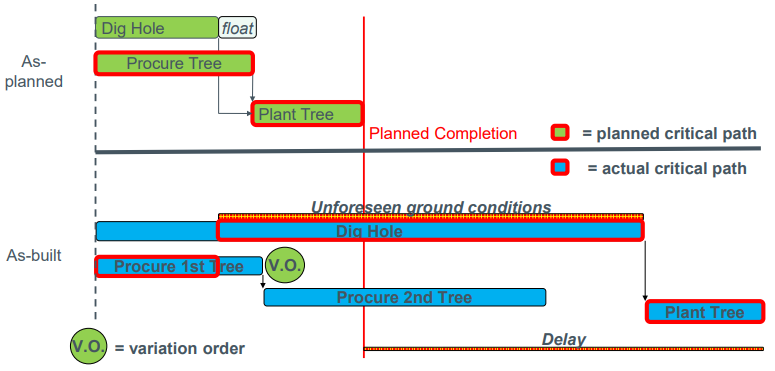
\includegraphics[width = \textwidth]{img/figure48.png}
    \caption{Comparison between planned and actual programmes.}
\end{figure}
Then the unhappy, but clever, instructing lawyer thinks:
\begin{quoting}
    ``That's all very well Mr Delay Expert, but what about the classic `but' for test of causation? Has there been an act of prevention here?''
\end{quoting}
\begin{figure}[H]
    \centering
    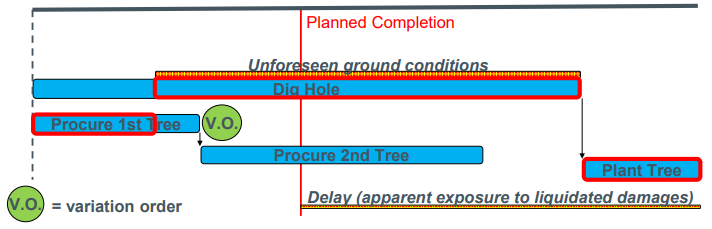
\includegraphics[width = \textwidth]{img/figure49.png}
    \caption{Critical path analysis.}
\end{figure}
\begin{figure}[H]
    \centering
    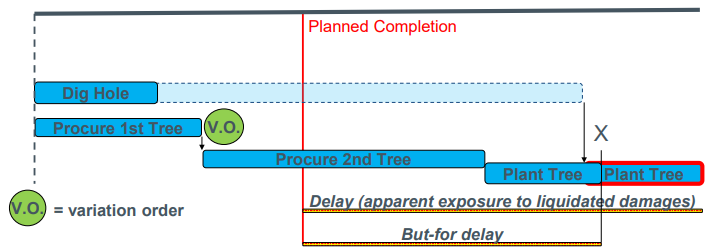
\includegraphics[width = \textwidth]{img/figure50.png}
    \caption{But-for delay.}
\end{figure}
\begin{quoting}
    ``Your honour, as a consequence of the instructed VO, there were no circumstances where my client could have completed this project any earlier than X. It would be harsh, indeed immoral, to expose her to Liquidated Damages liability before that date!''
\end{quoting}
\begin{figure}[H]
    \centering
    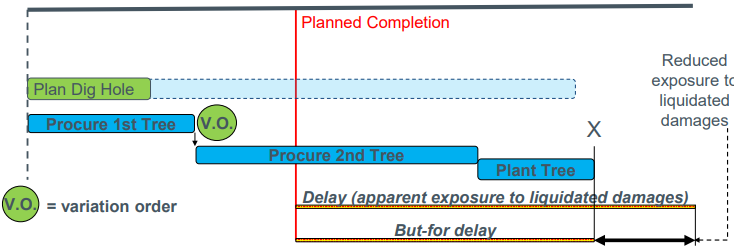
\includegraphics[width = \textwidth]{img/figure51.png}
    \caption{Reduced exposure to liquidated damages.}
\end{figure}
\section{Summary}
\begin{enumerate}
    \item The \textbf{delay expert} advises how the project was delayed
    \item The \textbf{technical expert} advises what technically went wrong
    \item The \textbf{quantum expert} advise on additional costs
    \item The \textbf{court} assigns liability and ultimately extension of time and damages
\end{enumerate}